\chapter{Methods}
\label{ch:methods}
This chapter outlines the methodology used to evaluate the performance of LLMs in classifying and transferring German texts by CEFR levels. It includes the dataset creation, benchmark design, model selection, data preparation and the fine-tuning process.

\section{Classification Dataset}
\label{s:dataset}
An integral part of any machine learning project is the dataset. Creating a dataset with German CEFR levels was challenging because there are no publicly available datasets with this information for all levels. I had to create a dataset from scratch, combining several existing datasets and using synthetic data generation to create a (balanced) dataset. It consists of about 1,500 texts, each ranging from 500 to 3,000 words. The texts are from different domains, such as simple texts, essays, summaries and more. There are all 6 CEFR levels in the dataset, ranging from A1 to C2. Additional preprocessing steps were taken to ensure the quality of the dataset, such as removing duplicates, removing non-valid characters and more.

\subsection{Creation of the Classification Dataset}
\label{ss:dataset_creation}
The classification dataset was created by integrating multiple existing datasets along with synthetic data generation to ensure a balanced composition. The FALKO Corpus \citep{reznicek2010falko} and MERLIN Corpus \citep{boyd2014merlin} used in this thesis are available under CC BY 3.0 and CC BY-SA 4.0 licenses respectively.
\subsubsection*{Falko Corpus}
\label{sss:falko_corpus}
A significant source utilized was the Falko corpus \citep{reznicek2010falko} collected and annotated at the Humbolt University Berlin. The corpus was designed to facilitate research in corpus linguistics by providing a collection of texts authored by both advanced foreign learners of German and native speakers, collected under controlled conditions and annotated for various linguistic features. From this corpus, the EssayL2, SummaryL1 and SummaryL2 subcorpora were selected due to them containing the necessary data. \\ \\
The \textbf{EssayL2} subcorpora consists of argumentative essays written by foreign learners of German with a CEFR level between B2 and C2. Topics include feminism, financial discussions and crime. All essays of the subcorpora were written under controlled conditions, with the learners having 90 minutes to write each essay. Each essay was then annotated with several metadata points such as the author's age, gender etc... Relevant to me was only the C-test score, which is an integer ranging from 0 to 100 to measure the author's German proficiency. The Falko authors gave a mapping to assign each C-test score to a CEFR level which I used to assign the CEFR level to each essay - see Table \ref{tab:ctest_mapping}.

\begin{table}[ht]
    \centering
    \begin{tabular}{
        >{\raggedright\arraybackslash}p{3cm}
        >{\raggedright\arraybackslash}p{3cm}
        }
        \toprule
        \textbf{Score Range} & \textbf{CEFR Level} \\
        \midrule
        60 - 79 & B2 \\
        80 - 89 & C1 \\
        90 - 100 & C2 \\
        \bottomrule
    \end{tabular}
    \caption{Mapping of C-Test Scores to CEFR Levels}
    \label{tab:ctest_mapping}
\end{table}

The \textbf{SummaryL1} and \textbf{SummaryL2} subcorporas consist of summaries of academic texts written by native speakers of German. The conditions were very similar to the EssayL2 subcorpora, with the learners having 90 minutes to write each summary. While the \textbf{SummaryL1} subcorpus contains summaries written by native speakers and thus processed as C2 samples for my dataset, the \textbf{SummaryL2} subcorpus includes summaries written by learners of German as a second language. \\

This dataset source was rather important as it contains a lot of native speaker texts, which are crucial for the model to understand the C2 level.

\subsubsection*{MERLIN Corpus}
\label{sss:merlin_corpus}
The second primary textual source was the MERLIN corpus \citep{boyd2014merlin}, a learner corpus designed to illustrate the CEFR with authentic learner data. It includes texts in three languages: Italian, Czech and German. There are entries covering all 6 CEFR levels with a strong focus on A2,B1 and B2 levels. Offering a diverse range of text types, including essays, summaries and other forms, the corpus is perfect for this thesis. These texts were collected as part of a standardized language test, which ensures the texts have great consistency and quality. All samples were annotated with CEFR levels by language experts, which guarantees the quality and accuracy of the labels. Due to that I could directly use the CEFR labeled texts provided by the corpus for my dataset.

\subsubsection*{Synthetic Data Generation}
\label{sss:synthetic_data_generation}
To address the scarcity of A1-level texts in the available sources, a synthetic data generation method was employed to enable having a dataset to evaluate across all CEFR levels.
I chose to use the Claude 3.5 Sonnet model \citep{claude3.5sonnet}, an advanced LLM developed by Anthropic due to its versatility in generating high-quality texts, large knowledge base and good prompt adherence \citep{Huang2024}.
The prompt engineering process consisted of several iterations to achieve the desired sample output. Initial attempts resulted in texts that showed a very high similarity to early primary school texts, which was not the desired outcome as I wanted texts in diverse topics to avoid dataset bias. Models would have associated the levels with the topics rather than the complexity of the text samples. To counteract these issues, I adjusted the prompt to avoid typical topics that the model would fall back to. Additionally the model was supplied a definition of the A1 level by the Goethe Institute to guide the model and prevent it from generating texts with higher complexity \citep{goetheCefr}. Also I settled on German as the language for the prompt as it showed better results than an English prompt. \\ \\
The final prompt used for the synthetic data generation was:
\captionsetup{labelformat=prompt}
\begin{figure}[h]
    \begin{quotation}
        \textit{Bitte generiere Texte mit dem CEFR Niveau A1. Diese sollten länger (Circa 600 Wörter) sein. Versuche Themen zu finden, welche nicht mit Schule/Kindheit in Verbindung stehen. Es sollte sich um Texte für Deutsch Sprachler mit dem Level A1 handeln. \\
        Hier ist eine Definition des A1 Levels: \\
        Kann vertraute, alltägliche Ausdrücke und ganz einfache Sätze verstehen und verwenden, die auf die Befriedigung konkreter Bedürfnisse zielen.
        Kann sich und andere vorstellen und anderen Leuten Fragen zu ihrer Person stellen – z. B. wo sie wohnen, welche Leute sie kennen oder welche Dinge sie haben – und kann auf Fragen dieser Art Antwort geben.
        Kann sich auf einfache Art verständigen, wenn die Gesprächspartner langsam und deutlich sprechen und bereit sind zu helfen.}
    \end{quotation}
    \caption{Final German Prompt for Synthetic Data Generation using definition by \cite{goetheCefr}}
    \label{qu:synthetic_prompt}
\end{figure}
\captionsetup{labelformat=default}

Using this I generated a total of 122 texts, which each undergoing a manual review to ensure  quality and relevance before being included in the dataset. \\ \\
While synthetic data generation proved effective for the A1 level, it was deemed unsuitable for the higher CEFR levels due to the complexity of the levels and the model's inability to reliably generate texts of that complexity. I am going to address this problem in the second part of my thesis (Section \ref{s:llm_fine_tuning}). There is also a risk of dataset bias, as the model could have generated texts with a schema that is not directly recognizable by humans. Regardless, this should not pose a problem in this case as the MERLIN dataset also provides A1 samples which were also used and thus the synthetic data is only a part of the dataset, not the whole dataset.

A detailed analysis of the dataset composition, distribution and word count across different CEFR levels is provided in the results chapter in Section \ref{s:classification_dataset_analysis}.

The transformation dataset for the transfer task is addressed later, as it relies on the fine-tuned classification model introduced in the following subsections. For details see Subsection \ref{ss:dataset_generation}.

\begin{table}[ht]
    \centering
    \begin{tabular}{
        >{\raggedright\arraybackslash}p{4cm}
        >{\raggedright\arraybackslash}p{1.25cm}
        >{\raggedright\arraybackslash}p{1.25cm}
        >{\raggedright\arraybackslash}p{1.25cm}
        >{\raggedright\arraybackslash}p{1.25cm}
        >{\raggedright\arraybackslash}p{1.25cm}
        >{\raggedright\arraybackslash}p{1.25cm}
        }
        \toprule
        \textbf{Source} & \textbf{A1} & \textbf{A2} & \textbf{B1} & \textbf{B2} & \textbf{C1} & \textbf{C2} \\
        \midrule
        Falko EssayL2     &     &     & & 83  & 84  & 81    \\ \midrule
        Falko SummaryL1   &     &     &     &  &    & 58   \\ \midrule
        Falko SummaryL2 & & & & & 53 & 53 \\ \midrule
        MERLIN            & 57  & 306 & 331 & 293 & 42 & 4  \\ \midrule
        Synthetic         & 122 &     &     &     &    &    \\ \midrule
        \textbf{Sum (1,567)}      & \textbf{179} & \textbf{306} & \textbf{331} & \textbf{376} & \textbf{179} & \textbf{196} \\
        \bottomrule
    \end{tabular}
    \caption{Data Distribution Across Different Levels}
    \label{tab:data_distribution}
\end{table}
\clearpage

\section{Evaluation Framework and Benchmark Design}
\label{s:evaluation_framework}
\subsection{Definition of Evaluation Metrics}
\label{ss:evaluation_metrics}
\subsubsection*{Classification Task}
\label{sss:classification_task}
Defining the evaluation metrics for the classification task is an important step to ensure the ability to judge the performance of the model and compare it to other models. This allows us to objectively measure the performance increase and the effectiveness of the prompts.
As this task is a very simple classification task (only 6 possible classes), I can use the standard evaluation metrics for classification tasks, consisting of accuracy, precision, recall and F1 score. See Table \ref{tab:common_evaluation_metrics} for a detailed explanation of the metrics.

\begin{table}[ht]
    \centering
    \begin{tabular}{
        >{\raggedright\arraybackslash}p{2cm}
        >{\raggedright\arraybackslash}p{6cm}
        >{\centering\arraybackslash}p{5cm}
        }
        \toprule
        \textbf{Metric} & \textbf{Description} & \textbf{Formula} \\
        \midrule
        Accuracy & Ratio of correctly classified samples to the total number of samples. Provides an overall measure of the model's performance across all classes. Can be misleading in cases of imbalanced datasets. & $\frac{\text{Number of Correctly Classified Samples}}{\text{Total Number of Samples}}$ \\
        \midrule
        Precision & Specific to each class. Ratio of correctly classified samples to the total number of samples classified as that class. Measures the model's ability not to label a sample as a certain class when it is not. & $\frac{\text{True Positives}}{\text{True Positives} + \text{False Positives}}$ \\
        \midrule
        Recall & Specific to each class. Ratio of correctly classified samples to the total number of samples that are actually in that class. Measures the model's ability to find all the samples that belong to a certain class. & $\frac{\text{True Positives}}{\text{True Positives} + \text{False Negatives}}$ \\
        \midrule
        F1 Score & Balances precision and recall, allowing comparison of models based on a single value. & $2 \cdot \frac{\text{Precision} \cdot \text{Recall}}{\text{Precision} + \text{Recall}}$ \\
        \bottomrule
    \end{tabular}
    \caption{Common Evaluation Metrics for Classification Tasks}
    \label{tab:common_evaluation_metrics}
\end{table}

Additionally to these standard metrics, I also introduced another metric called \textit{group accuracy}. As CEFR classifications are inherently subjective due to their language origin \citep{Siddhant2020} and the boundaries between levels are not always clear, it is possible, that different experts classify the same text differently. Therefore there could be a situation where a text is classified as B1 but also as B2 - both classifications could be correct. To account for this, I introduced the group accuracy metric. I define a group as a set of two adjacent CEFR levels. For example, a group consists of A1 and A2, another group of A2 and B1 and so on. The group accuracy is then defined as the ratio of samples that were classified in the correct group to the total number of samples - allowing to measure the model's ability to classify texts in the correct group, even if the exact level is not correct.

\subsubsection*{Transfer Task}
\label{sss:transfer_task}
For the transfer task, the evaluation metrics are substantially more complex. The model is evaluated on its ability to transfer knowledge from one CEFR level to another while retaining the content. Evaluation metrics for this task are two fold:
To begin with, the transferred text undergoes classification to determine if it matches the target CEFR level utilizing the classification LLM. By using the classifier, I ensure a consistent and reliable metric for evaluation. Additionally I determine the group transfer accuracy, similar to the classification task.
% The transferred text's CEFR level is determined using the previously developed classification model. This approach provides a consistent and reliable metric for evaluating the transfer process's accuracy in achieving the target CEFR level.
Secondly, the content retention is evaluated by employing a second (foundation) LLM as a judge model. The LLM is given the original and transferred text while being tasked to evaluate the content similarity between the two texts.
% Only if the target CEFR level is reached and the content is retained, the transfer is considered successful.

\begin{table}[ht]
    \centering
    \begin{tabular}{
        >{\raggedright\arraybackslash}p{2cm}
        >{\raggedright\arraybackslash}p{7cm}
        >{\centering\arraybackslash}p{4cm}
        }
        \toprule
        \textbf{Metric} & \textbf{Description} & \textbf{Methodology} \\
        \midrule
        Transfer accuracy & Ratio of samples where the transferred text is classified as the target CEFR level to the total number of samples. & Classification LLM \\
        \midrule
        Group Transfer accuracy & Ratio of samples where the transferred text is classified as the target CEFR level or the adjacent CEFR level to the total number of samples. & Classification LLM \\
        \midrule
        Content Preservation Rate & Ratio of samples where the content similarity between the original and the transferred text is sufficiently retained, as evaluated by a LLM, to the total number of samples. & Judge LLM \\  \bottomrule
    \end{tabular}
    \caption{Evaluation Metrics for Transfer Tasks}
    \label{tab:evaluation_metrics}
\end{table}

\subsection{Classification Task Benchmark Design}
\label{ss:benchmark_design}
The benchmark for the classification task is designed to evaluate the performance of the classification LLM. In the following, I will define a run as a single evaluation cycle of the model. For each run, a given amount of samples for each CEFR level are selected. Then, using a base model with prompting, the samples are randomly selected from the dataset. If a fine-tuned model is being benchmarked, the samples are selected from the validation split of the dataset for that specific model.

For each sample, the model is tasked to classify the text. The system prompt is set to an instruction and the sample is supplied to the model as the first user message. The model then generates the second message, which is the classification of the text with a limit of 2 tokens.
After the model has generated all predictions, the evaluation metrics are calculated for the whole run (accuracy and group accuracy) and each CEFR level (precision, recall and F1). This process can be repeated multiple times to get a more accurate representation of the model's performance, as with a temperature > 0 the model will generate different outputs for the same input. Final evaluation metrics are then calculated as the average over all runs. For this thesis, I decided on a temperature of 0 for the classification task as this guarantees consistent results. Additionally, testing showed the models seems to perform better with a temperature of 0. This makes sense due to the model only having to generate two tokens, which would be massively skewed by a higher temperature. Additionally this choice also provides reproducibility, as the results are consistent across runs.

Accompanying the benchmark, I developed a small web interface to allow for easy testing of the model. The interface allows the user to select a model and benchmark parameters such as the number of runs, temperature, sample size, system prompt and more. It then automatically runs the benchmark and displays the runs in an easy to read list. For each run the user can access a detailed view, showing the run results in a confusion matrix and the evaluation metrics for each CEFR level. This allows for easy and fast comparison of different models and benchmark parameters. Additionally, the interface has some additional features such as the ability to abort runs that result in a lot of miss-classifications in direct succession, indication an issue with the model or prompt. \\


\section{CEFR Classification via Prompt Engineering}
\label{s:prompt_engineering}
\subsection{Prompt Design Strategy}
\label{ss:prompt_design}
I started the prompt design process by choosing a first base model to start working with to evaluate my prompts. This choice turned out to be the LLaMA3-8B model \citep{LLaMA3} as it is rather small and thus has fast inference times, allowing for quick testing of prompts. Later on I chose the best performing model, see Subsection \ref{ss:base_model_selection}. The prompt design process was iterative and consisted of several steps, each improving on the previous one. With the end goal being to design a prompt that instructs the model to effectively classify the CEFR level of a given text.

\subsubsection*{Basic Prompt}
\label{sss:basic_prompt}
Initial steps involved designing a simple prompt instructing the model to classify the first text supplied by the user in the conversation. Two parts are integral to the prompt: First a simple description of the model's task and secondly a list of valid responses for the model to chose from. I decided first try to design the prompt in English, as the model was mostly trained on English data \citep{LLaMA3} and that should lead to better instruction adherence. Similar behavior is common in LLMs as shown by \cite{Siddhant2020}. The performance of this prompt was evaluated, with results available in the appendix \ref{tab:first_english_prompt}.
\captionsetup{labelformat=prompt}
\begin{figure}[h]
    \begin{quotation}
        \textit{Classify the language level of a given text according to the Common European Framework of Reference for Languages (CEFR). Respond with only the corresponding CEFR level (A1, A2, B1, B2, C1 or C2).}
    \end{quotation}
    \caption{First English Prompt}
    \label{qu:first_english_prompt}
\end{figure}
\captionsetup{labelformat=default}

\subsubsection*{German Zero-Shot Prompt}
\label{ss:german_zero_shot_prompt}
The evaluation of the previous prompt showed some problems. To address these shortcomings, a switch to German was made, based on two considerations:
\begin{enumerate}
    \item First, as the classification task is designed for German texts, using a German prompt could potentially profit from more relevant language knowledge in the model. Also as German has the same origin as English, the languages share some similarities. \cite{Pires2019} has shown, that LLMs can better adapt to languages, that are similar to the ones they were mostly trained on. So this could potentially lead to better results.
    \item Secondly, the model had already shown good adherence to instructions, suggesting that the problem remains in the classification task itself rather than in understanding and following the prompt.
\end{enumerate}
The new prompt is a direct translation of the English prompt, with minor adjustments to ensure natural phrasing in German and a focus on the valid responses.
\captionsetup{labelformat=prompt}
\begin{figure}[h]
    \begin{quotation}
        \textit{Bewerte die Sprachkenntnisse des bereitgestellten deutschen Textes gemäß dem Gemeinsamen Europäischen Referenzrahmen für Sprachen (GER/CEFR). Antworte NUR mit der entsprechenden Stufe: A1, A2, B1, B2, C1 oder C2, *keiner* Begründung}
    \end{quotation}
    \caption{German Zero-Shot Prompt}
    \label{qu:german_prompt}
\end{figure}
\captionsetup{labelformat=default}

The effectiveness of this German prompt was assessed through comparative testing against its English counterpart showing slight improvement in the model's performance. See the appendix Table \ref{tab:zero_shot_confusion_matrix} for the results.

% This lead to a small improvement in the model's performance, with the overall accuracy increasing to 33.3\% and the group accuracy rising to 75.3\%. The model started to show substantial improvements in classifying A1-A2 and C1-C2 levels. However there still was a rather string bias towards the B1 and B2 levels, albeit less pronounced than with the English prompt. This persistent bias might be attributed to these intermediate levels representing a "middle ground" in language proficiency, making them harder to distinguish from adjacent levels.
% While the German prompt showed promise, the accuracy levels were still not good enough. This led to the exploration of more advanced prompting techniques, as discussed in the following section.

\subsubsection*{German Few-Shot Prompt}
\label{ss:few_shot_prompt}
For now all prompts were zero-shot prompts, meaning that the model was not given any examples with desired output beforehand. To further increase performance, a few-shot prompt was designed, where the model is given a few text samples with their corresponding CEFR level. 
As shown by \cite{Brown2020}, this should help the model to better understand the task and improve its performance. The few-shot prompt can be seen in Prompt \ref{qu:few_shot_prompt}.

\captionsetup{labelformat=prompt}
\begin{figure}[h]
    \begin{quotation}
        \textit{Klassifiziere die Sprachkenntnisse des bereitgestellten deutschen Textes gemäß dem Gemeinsamen Europäischen Referenzrahmen für Sprachen (GER/CEFR). Antworte NUR mit der entsprechenden Stufe: A1, A2, B1, B2, C1 oder C2, NICHT MEHR. Gebe auch *keine* Begründung! \\
        Hier sind jeweils Beispiele: \\ \\
        A1: Lieber Jens, Ich Glückwünsche dich ist Vater geworden. Wie es deine Frau und deine Babys? Wie heißt des Babys? Brauchst du etwas hilfe? Könntest du bitte mich anrufen? Herzlichen Grüßen Maria Meier \\
        A2: [...] \\
        B1: [...] \\
        B2: [...] \\
        C1: [...] \\
        C2: [...]}
    \end{quotation}
    \caption{German Few-Shot Prompt, shortened (See Prompt \ref{qu:few_shot_prompt_complete} for full version)}
    \label{qu:few_shot_prompt}
\end{figure}
\captionsetup{labelformat=default}

For readability reasons I only included the A1 example in the prompt, the other examples are similar in structure and content. Also note that the grammar and spelling mistakes are intentional, as they are typical for the respective CEFR level and the sample was taken from a real text. See the appendix at Prompt \ref{qu:few_shot_prompt_complete} for the full version.

This prompt incorporates an example with its corresponding class for each CEFR level. All examples were specifically selected from samples that the model had previously misclassified, with the aim of enhancing the model's understanding of the task and improving its performance. \\
% TODO: move to results
% The few-shot prompt showed a significant improvement in the model's accuracy, which increased to 59.3\%, while the group accuracy rose to 94.0\%. Additionally, the bias towards the B1 and B2 levels was also reduced. However, the model still showed difficulties with classifying texts at the A2 and C1 levels, as shown in Table \ref{tab:few_shot_confusion_matrix}. These persistent problems with A2 and C1 classifications may stem from them being between the two endpoints and middle levels. While it is relatively easy to distinguish between very simple, medium, and highly complex texts (corresponding to A1, B1/B2, and C2 levels respectively), the differences in the middle levels are harder to distinguish.
Additional experimentation with prompting did not yield any further improvements in accuracy. Notably, the inclusion of additional examples in the prompt did not result in significant improvements - in fact, it led to a slight decrease in classification accuracy. This effect may be caused by potential overfitting, where the model becomes too closely aligned with the specific examples provided in the prompt, potentially hampering its ability to generalize to new, unseen texts. 

\subsection{Base Model Selection}
\label{ss:base_model_selection}
\subsubsection*{Selection Criteria}
\label{sss:selection_criteria}
After refining the prompt with a stand-in model I decided to evaluate different models to find the best one. Before deciding on a model, I first had to define the selection criteria. \\
The most important criterion was the model's performance on the classification task, mainly the accuracy and group accuracy scores.
Additionally the model's parameter count and inference time were also considered for two reasons. Firstly, a small(er) model (<30B parameters) would allow for faster inference times, thus being more effective and practical for real world use. Secondly, a smaller model would also be easier to fine-tune, as it requires less computational resources.  \\
% This is not as important for the classification task, but becomes crucial for the transfer task, where a fine-tuning step is likely to be performed. \\
Lastly, the model's adherence to the prompt was also considered. For the classification task the model needs to only respond with the CEFR level, nothing else. If the models does not adhere to the prompt and provides additional information or argumentation, it is considered a wrong classification and results in worse performance. \\
Also important was, that the model has open weights and can be fine-tuned. This criteria includes the right license for research fine-tuning.

\subsubsection*{Possible Models}
\label{sss:possible_models}
The following models were considered for evaluation:
% \begin{itemize}
%     \item Meta-LLaMA-3-8B-Instruct \cite{LLaMA3}
%     \item Meta-LLaMA-3-70B-Instruct \cite{LLaMA3}
%     \item Mistral-7B-Instruct \cite{Jiang2023}
%     \item Mixtral-8x22B-Instruct-v0.1 \cite{Jiang2023}
%     \item google/gemma-2-9b-it \cite{GemmaTeam2024}
%     \item google/gemma-2-27b-it \cite{GemmaTeam2024}
%     \item qwen/qwen2-7B-Instruct \cite{Yang2024}
%     \item qwen/qwen2-72B-Instruct \cite{Yang2024}
% \end{itemize}
\begin{table}[ht]
    \centering
    \begin{tabular}{
        >{\raggedright\arraybackslash}p{5cm}
        >{\arraybackslash}p{4.5cm}
        }
        \toprule
        \textbf{Model Name} & \textbf{Reference} \\
        \midrule
        Meta-LLaMA-3-8B-Instruct & \cite{LLaMA3} \\
        \midrule
        Meta-LLaMA-3-70B-Instruct & \cite{LLaMA3} \\
        \midrule
        Mistral-7B-Instruct & \cite{Jiang2023} \\
        \midrule
        Mixtral-8x22B-Instruct-v0.1 & \cite{Jiang2023} \\
        \midrule
        google/gemma-2-9b-it & \cite{GemmaTeam2024} \\
        \midrule
        google/gemma-2-27b-it & \cite{GemmaTeam2024} \\
        \midrule
        qwen/qwen2-7B-Instruct & \cite{Yang2024} \\
        \midrule
        qwen/qwen2-72B-Instruct & \cite{Yang2024} \\
        \bottomrule
    \end{tabular}
    \caption{Language Models Considered for Evaluation}
    \label{tab:llm_models}
\end{table}

% \subsubsection*{Selected Model}
% \label{sss:selected_model}
% After evaluating all models based on their performance, size and license, I determined the Meta-LLaMA-3-8B-Instruct model to be the best choice for the classification task and further fine-tuning. For further results see the appendix \ref{tab:base_model_selection}.

\subsubsection*{Selected Model}
\label{sss:selected_model}
After evaluating all models based on their performance, size and license, I determined the Meta-LLaMA-3-8B-Instruct model to be the best choice for the classification task and further fine-tuning. The selection process considered several key factors:

\begin{enumerate}
    \item Performance: The model's accuracy and group accuracy were evaluated on a subset of the dataset. While specific results are presented in the Results section at \ref{fig:llm-performance-comparison}, the LLaMA-3-8B-Instruct model demonstrated competitive performance.
    \item Model Size: With 8 billion parameters, this model offers a good balance between capability and computational efficiency. This was an important consideration for both fast inference speed and the ability to fine-tune the model effectively and iterate quickly.
    \item Open Weights: The availability of open weights was crucial for this thesis, as it allows for fine-tuning and adaptation to the specific tasks.
    \item Licensing: The model's license permits research use and fine-tuning, which aligns with this thesis needs.
    \item Architecture: The LLaMA-3-8B-Instruct model uses a transformer architecture optimized for instruction following, which is well-suited for the classification and transfer tasks.
\end{enumerate}

While larger models were available, the LLaMA-3-8B-Instruct model offered the best compromise between performance and resource requirements. The detailed performance comparisons that led to this selection, including accuracy and group accuracy metrics for all evaluated models can be found in the appendix at \ref{fig:llm-performance-comparison}.

It is important to mention, that the model selection process has a slight bias towards the LLaMA-3-8B-Instruct model. As the evaluation of the different models was done on the manually refined prompt, which was designed with the LLaMA-3-8B-Instruct model as a stand-in. This could potentially lead to a bias towards this model, as the prompt was iteratively designed to work well with this model. It could be, that with other prompts the results would be different and another model would be better contenders. As the prompt showed good results with several other models as well, the bias should be minimal but still needs to be mentioned and kept in mind.
\section{CEFR Classification via LLM Fine-Tuning}
\label{s:llm_fine_tuning}

After exploring prompting for the classification task, I moved on to fine-tuning a model on the classification task to see if this would lead to better results. Fine-tuning involves further training of an already pre-trained model on a dataset to adapt the model to a specific task or domain. This will allow the model to learn patterns and features relevant to the CEFR classification task. In this section I will discuss dataset preparation and the process of fine-tuning itself.

\subsubsection{Model Selection}
\label{sss:model_selection}
Based on Subsection \ref{ss:base_model_selection} I decided to fine-tune the Meta-LLaMA-3-8B-Instruct model. This model showed the best performance on the classification task and adhered well to the prompt. Additionally, the model has a relatively small parameter count, which should allow for faster fine-tuning and inference times. LLaMA3 also has open weights and is licensed for research fine-tuning \citep{LLaMA3}.

\subsubsection{Dataset Preparation}
\label{sss:dataset_preparation}
To prepare the dataset I first randomly selected 179 samples from each CEFR level. This was done do avoid any bias towards the center levels as these were overrepresented in the dataset (See Table \ref{tab:data_distribution}) and 179 samples is the lowest number of samples for a CEFR level. The samples were then split into two parts:
\begin{itemize}
    \item Training data: 154 per CEFR level to be used for fine-tuning the model
    \item Test data: 25 samples per CEFR level to be used for evaluation of the fine-tuned model
\end{itemize}
All texts were formatted for the fine-tuning process. Each sample was formatted as a single string that conforms to the LLAMA 3 input format, consisting of a system prompt, a user message and the assistant response separated by special tokens. 
Special tokens are tokens that are not part of the normal text embedding vocabulary and used to separate the different parts of the input and indicate end of the models response. A shortened version of the prompt used for the classification task was used as the system prompt, removing the examples for each CEFR level as they will be implicitly learned by the model during fine-tuning. The first user message was set to the sample to be classified by the model. Then the assistant response was set to the correct CEFR level. See Prompt \ref{qu:formatted_sample} for an example of a formatted sample.

\captionsetup{labelformat=prompt}
\begin{figure}
    \begin{quotation}
        \textcolor{gray}{<|start\_header\_id|>}\textcolor{blue}{system}\textcolor{gray}{<|end\_header\_id|>}Klassifiziere das Sprachniveau des bereitgestellten deutschen Textes gemäß dem Gemeinsamen Europäischen Referenzrahmen für Sprachen (GER/CEFR). Antworte NUR mit der entsprechenden Stufe: A1, A2, B1, B2, C1 oder C2, NICHT MEHR.\textcolor{gray}{<|eot\_id|>}\textcolor{gray}{<|start\_header\_id|>}\textcolor{blue}{user}\textcolor{gray}{<|end\_header\_id|>}\textcolor{orange}{[SAMPLE]}
        \textcolor{gray}{<|eot\_id|>}\textcolor{gray}{<|start\_header\_id|>}\textcolor{blue}{assistant}\textcolor{gray}{<|end\_header\_id|>}\textcolor{orange}{[CORRECT SAMPLE CLASS]}\textcolor{gray}{<|eot|>}
    \end{quotation}
    \caption{Formatted Prompt Sample for Fine-Tuning}
    \label{qu:formatted_sample}
\end{figure}
\captionsetup{labelformat=default}

Then all formatted samples were scrambled to avoid any problems in the training process due to class repetition.

\subsubsection{Fine-Tuning Process}
\label{sss:fine_tuning_process}
The fine-tuning process was conducted using Unsloth, which is specifically designed for efficient fine-tuning of LLMs. Training was carried out on an NVIDIA GPU, leveraging PyTorch for the underlying computations.
I used llama-3-8b-Instruct as the base model, with a maximum sequence length of 4096 tokens. The model was loaded in 16-bit precision (float16) to achieve best computational accuracy. To ensure efficient resource usage for the fine-tune I employed Low-rank Adaptation with a rank of 64 and a dropout of 0.

The following hyper-parameters were used for the fine-tuning itself:

\begin{table}[ht]
    \centering
    \begin{tabular}{ll}
        \toprule
        \textbf{Hyperparameter} & \textbf{Value} \\
        \midrule
        Learning rate & 2e-4 \\
        Number of epochs & 5 \\
        Batch size & 1 \\
        Gradient accumulation steps & 1 \\
        Warmup steps & 400 \\
        Weight decay & 0.001 \\
        Learning rate scheduler & Linear \\
        \bottomrule
    \end{tabular}
    \caption{Hyperparameter Used for Fine-tuning}
    \label{tab:fine_tuning_hyperparameters}
\end{table}
The learning rate of 2e-4 was chosen as it is recommended by the Unsloth authors as a good starting point for fine-tuning LLMs, balancing between learning speed and stability \citep{unsloth2024}. I ran the training for 5 epochs, which was determined to be sufficient for the model to converge on the task without overfitting, based on previous experiments. These showed that the loss was not decreasing significantly after the 5th epoch. Additionally, there was no increase in performance for these runs. I chose a batch size of 1 as I wasn't constrained by memory with the 8B parameters of the model. For the optimizer I chose the AdamW optimizer in the 8-bit variant. AdamW is an extension of the Adam optimizer that implements decoupled weight decay regularization, which can help with reducing overfitting \citep{Loshchilov2017}. I chose not to implement any additional overfitting protection, as previous experiments showed no real danger of that occurring with the 5 epochs chosen for this fine-tuning approach.

The fine-tuning was performed on an NVIDIA RTX A6000 GPU. This GPU has 48GB of VRAM, which was sufficient for fine-tuning the 8B parameter model. The process was implemented using PyTorch \citep{Paszke2019} as the underlying framework, with Unsloth providing optimizations specific to LLM fine-tuning. Fine-tuning took approximately 20 minutes to complete the 5 epochs. During training the loss and learning rate were monitored to avoid overfitting and ensure an efficient training.

In the end the LoRa adapter was merged with the base model to create the final fine-tuned model with 16bit precision. This model was then evaluated on the test data to determine its performance on the classification task. Results of this evaluation are presented in the results section at \ref{sss:best_finetuning_evaluation}.

\section{Text Adaptation through LLM Fine-Tuning}
\label{s:llm_fine_tuning}
\subsection{Dataset Generation}
\label{ss:dataset_generation}
The existing dataset created in Subsection \ref{sss:dataset_preparation} contained only the original text samples and their corresponding CEFR levels. To do the transfer task fine-tuning I needed to create a new dataset that contained the text samples in multiple CEFR levels. As it was not practical to manually create such a dataset, I decided to use synthetic data generation. In the initial dataset generation step, this was not possible due to the inability to correctly classify generated data. Despite this, with the fine-tuned model from \ref{sss:fine_tuning_process}, I was able to use a different approach. \\

\begin{figure}[h]
    \centering
    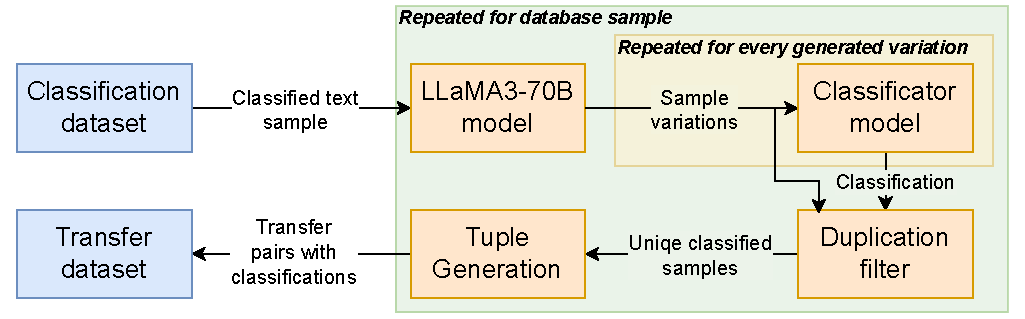
\includegraphics[width=\textwidth]{img/TransferDatasetCreation2.pdf}
    \caption{Dataset Generation Process for Text Adaptation}
    \label{fig:dataset_generation_process}
\end{figure}

\subsubsection*{Dataset Generation Process}
\label{sss:dataset_generation_process}
I ended up using another foundation model to generate the synthetic data and verify the correct classification using the fine-tuned model.
The generation process began by iterating trough all samples in the original dataset to serve as a "base" sample for adaptation. For every base text, I instructed a base LLaMA3-70B model (See Prompt \ref{qu:adaptation_prompt}) to generate adapted versions of the base sample in all CEFR levels while preserving the original content and meaning. This approach was designed to maintain consistency in the content across different proficiency levels. The model was specifically directed to produce all versions at once, a strategy that allowed it to consider the context of lower-level transformations while generating higher-level versions. Ensuring a coherent progression in language complexity across the CEFR levels.

\captionsetup{labelformat=prompt}
\begin{figure}[h]
    \begin{quotation}
        \textit{
            Erstelle bitte Varianten des folgenden Textes in allen CEFR Niveaus, außer dem Originalniveau \textcolor{orange}{[ORIGINAL LEVEL]}: \\ \\
            "\textcolor{orange}{[SAMPLE TEXT]}" \\ \\
            Die Texte sollten den gleichen Inhalt haben, aber an das jeweilige CEFR Niveau angepasst sein. Gebe die Texte als JSON Objekt mit CEFR-Leveln als Keys zurück und antworte NUR mit dem Objekt, keine Begründungen, keine Codeblöcke(```), keine Erklärungen dass du etwas nur versuchen kannst oder ähnliches! Und stelle sicher, dass die Texte den gleichen Inhalt haben, sonst wirst du gefeuert!
        }
    \end{quotation}
    \caption{Prompt for Broad Text Adaptation}
    \label{qu:adaptation_prompt}
\end{figure}
\captionsetup{labelformat=default}

After the generation, each newly generated sample underwent classification by the fine-tuned model, ensuring the correct classification of the generated samples the quality of the new dataset. The samples were then filtered to remove multiple transformed samples in the same CEFR level. As a final step, all possible combinations of two-pair samples were generated, including bidirectional transformations. This was done to ensure that the model would be exposed to a diverse range of CEFR level transitions during training.

See Table \ref{tab:transfer_distribution} for an overview of the distribution of the generated samples.

\begin{table}[ht]
    \centering
    \begin{tabular}{
      >{\raggedright\arraybackslash}p{2.5cm}
      >{\raggedright\arraybackslash}p{2cm}
      >{\raggedright\arraybackslash}p{2cm}
    }
        \toprule
        \textbf{Transfer Type} & \textbf{Count} & \textbf{Percentage} \\
        \midrule
        A1 $\leftrightarrow$ C1 & 250 & 20.63\% \\
        A1 $\leftrightarrow$ C2 & 236 & 19.47\% \\
        A2 $\leftrightarrow$ C2 & 174 & 14.36\% \\
        A2 $\leftrightarrow$ C1 & 160 & 13.20\% \\
        A1 $\leftrightarrow$ B2 & 126 & 10.40\% \\
        A1 $\leftrightarrow$ B1 & 66 & 5.45\% \\
        A2 $\leftrightarrow$ B2 & 64 & 5.28\% \\
        B1 $\leftrightarrow$ C1 & 54 & 4.46\% \\
        B1 $\leftrightarrow$ C2 & 46 & 3.80\% \\
        B2 $\leftrightarrow$ C2 & 14 & 1.16\% \\
        A2 $\leftrightarrow$ B1 & 10 & 0.83\% \\
        B2 $\leftrightarrow$ C1 & 8 & 0.66\% \\
        A1 $\leftrightarrow$ A2 & 4 & 0.33\% \\
        \midrule
        \textbf{Total entries} & \textbf{1212} & \textbf{100\%} \\
        \bottomrule
    \end{tabular} \\
    \textit{Note: Bidirectional transformations are combined for better readability. See Table \ref{tab:detailed_transfer_distribution} for a detailed version.} \\
    \caption{Transfer Distribution Overview}
    \label{tab:transfer_distribution}
\end{table}

\phantom{} % Needed as LaTeX breaks without it and some figures disappear into a digital abyss. Idk why, but it works this way.

\subsection{Fine-Tuning Preparation // Dataset Preparation}
\label{ss:fine_tuning_preparation}
After generating the synthetic dataset with multiple CEFR levels for each original sample, I prepared the data for the fine-tuning process. This preparation involved several key steps to ensure the integrity and balance of the training and test sets.

The first step in the preparation process was bidirectional grouping. The dataset contains bidirectional transformations (e.g., A1->C1 and C1->A1) for each pair generated from the original samples. To prevent potential contamination between training and test sets, these bidirectional transformations were grouped together. By doing so, related transformations are treated as a unit throughout the preparation and splitting process.

Following the bidirectional grouping, I used a level pair balancing strategy. The transformations were grouped by CEFR level pairs (e.g., A1->C1, B1->C2). To ensure a balanced representation of all level pairs, I set minimum and maximum limits for the number of samples in each pair. This helps to prevent bias towards certain level transformations and ensures that the model is exposed to a diverse range of CEFR level transitions during training.

With the dataset grouped and balanced, I split it into training and test sets. The split was designed to maintain the integrity of the bidirectional groups by keeping those always together. Approximately 80\% of the samples were allocated to the training set, to be used for fine-tuning the model. Importantly, this set includes at least one sample from each CEFR level pair, ensuring complete coverage during training. The remaining 20\% of the samples were used as the test set.

For the transfer task, I designed a specific user prompt template to instruct the model to adapt the text to a specific CEFR level. The prompt was crafted to be clear, concise and explicit in its instructions to ensure the model's adherence to the task.
% The German language was chosen for the prompt to maintain consistency with the task of transforming German texts.
% The prompt template is shown in Prompt \ref{qu:single_adaptation_prompt}.
\captionsetup{labelformat=prompt}
\begin{figure}[h]
    \begin{quotation}
        \textit{
            Übersetze den folgenden deutschen Text auf das CEFR-Sprachniveau \textcolor{orange}{[TARGET LEVEL]}, während du den ursprünglichen Inhalt und die Bedeutung so weit wie möglich beibehältst: \\ \\
            \textcolor{orange}{[ORIGINAL TEXT]}
        }
    \end{quotation}
    \caption{Prompt for Text Adaptation}
    \label{qu:single_adaptation_prompt}
\end{figure}
\captionsetup{labelformat=default}

% It was designed to clearly specify the target CEFR level, emphasize the importance of maintaining the original content and meaning, and providing a clear structure for the model to follow.

Each sample consisting of an original text, transferred text, original level and target level was then formatted into a format suitable for fine-tuning the LLaMA3 model. The format was the same as in Section \ref{s:llm_fine_tuning} and used the Prompt \ref{qu:single_adaptation_prompt} for the first user message. See Prompt \ref{qu:formatted_adaptation_sample} for an template of a formatted sample.

\subsection{Fine-Tuning Process}
\label{ss:fine_tuning_process}
The fine-tuning was conducted using the same setup as in Section \ref{sss:fine_tuning_process}. Most hyperparameter were kept the same, with the two differences being that the model was only trained for 3 epochs and on a different dataset. This was determined to be sufficient for the model to adapt to the new task without overfitting as the dataset was rather small due insufficient data sources. Completing the fine-tuning process took approximately 10 minutes. The final fine-tuned model was then evaluated on the test data using the metrics defined in \ref{sss:transfer_task}. Results of this evaluation are presented in the results section \ref{sss:best_finetuning_evaluation}.

\captionsetup{labelformat=prompt}
\begin{figure}[h]
    \begin{quotation}
        \textit{
            \textcolor{gray}{<|start\_header\_id|>}\textcolor{blue}{system}\textcolor{gray}{<|end\_header\_id|>}Transformiere den gegebenen deutschen Text auf das angegebene CEFR-Niveau, während du die ursprüngliche Bedeutung beibehältst.\textcolor{gray}{<|eot\_id|>} \\
            \textcolor{gray}{<|start\_header\_id|>}\textcolor{blue}{user}\textcolor{gray}{<|end\_header\_id|>}\textcolor{orange}{[USER PROMPT]}Ziel-CEFR-Niveau: \textcolor{orange}{[TARGET NIVEAU]}\textcolor{gray}{<|eot\_id|>} \\
            \textcolor{gray}{<|start\_header\_id|>}\textcolor{blue}{assistant}\textcolor{gray}{<|end\_header\_id|>}\textcolor{orange}{[TRANSFERRED TEXT]}\textcolor{gray}{<|eot\_id|>}
            }
        \end{quotation}
        \caption{Formatted Prompt Sample for Fine-Tuning}
        \label{qu:formatted_adaptation_sample}
\end{figure}
\captionsetup{labelformat=default}

\subsection{Benchmark Design}
\label{sss:transfer_benchmark}
The transformation benchmark was designed to evaluate the model's ability to adapt German texts between different CEFR levels while maintaining content integrity, utilizing both the fine-tuned transfer model and the classification model.

\begin{figure}[h]
    \centering
    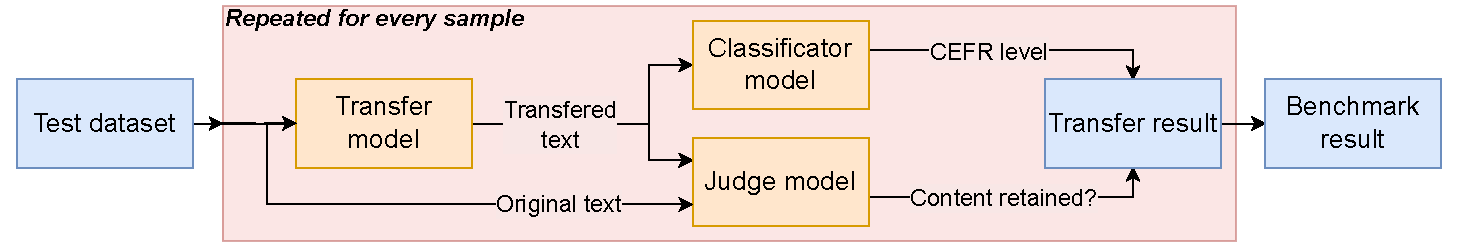
\includegraphics[width=\textwidth]{img/TransferBenchmark3.pdf}
    \caption{Transfer Benchmark Design}
    \label{fig:transfer_benchmark}
\end{figure}

The test dataset consists of samples containing original texts, their CEFR levels and target levels for transformation. For each sample, the original text and target CEFR level are fed into the transfer model using the adapted Prompt \ref{qu:single_adaptation_prompt}.
The model then generates a transformed version of the text, aiming to match the target level. This generated text is then classified using the classification model. To assess content preservation, a separate "judge" model evaluates the similarity between the original and transformed texts. For that I designed Prompt \ref{qu:content_retention_prompt}. I selected LLAMA-3-70B-Instruct \citep{LLaMA3} as the judge model, as it showed promising results in previous experimental testing.

\captionsetup{labelformat=prompt}
\begin{figure}[h]
    \begin{quotation}
        \textit{Original: \textcolor{orange}{[ORIGINAL TEXT]} \\
        Transferred: \textcolor{orange}{[TRANSFERRED TEXT]} \\
        Haben diese beiden Texte das gleiche Thema und selben Inhalt? Antworte nur mit 'Ja' oder 'Nein'.}
    \end{quotation}
    \caption{Content retention prompt}
    \label{qu:content_retention_prompt}
\end{figure}
\captionsetup{labelformat=default}

After all test samples were processed, the evaluation metrics are calculated. This includes the transformations transfer accuracy, group transfer accuracy and content preservation scores. All results of this benchmark are presented and evaluated in the following results Section \ref{s:transfer_results}.